\documentclass[11pt,a4paper,oneside]{article}

\usepackage{tikz}
\usetikzlibrary{shapes,positioning}
\definecolor{darkgreen}{rgb}{0,0.5,0}

% Schrift
\usepackage[utf8]{inputenc}
\usepackage[T1]{fontenc} 
\usepackage{lmodern}
%\usepackage{textcomp}

% Dokument in deutsch
\usepackage{ngerman}
%\usepackage[ngerman]{babel} 

\definecolor{clBlue}{rgb}{.122,.286,.490}
\definecolor{clChapTxt}{rgb}{.090,.212,.365}
\newcommand{\parspace}{\setlength{\parskip}{10pt}}
% Zeilenabstand
\linespread{1.15}

\makeatletter
\renewcommand{\section}{\@startsection {section}{1}{\z@}%
                                   {-3.5ex \@plus -1ex \@minus -.2ex}%
                                   {2.3ex \@plus.2ex}%
                                   {\rmfamily\Large\bfseries\boldmath\color{clBlue}}}
\renewcommand{\subsection}{\@startsection{subsection}{2}{\z@}%
                                     {-3.25ex\@plus -1ex \@minus -.2ex}%
                                     {1.5ex \@plus .2ex}%
                                     {\rmfamily\large\bfseries\boldmath\color{clBlue}}}
\renewcommand{\subsubsection}{\@startsection{subsubsection}{3}{\z@}%
                                     {-3.25ex\@plus -1ex \@minus -.2ex}%
                                     {1.5ex \@plus .2ex}%
                                     {\rmfamily\normalsize\bfseries\boldmath\color{clBlue}}}
\def\@makechapterhead#1{%
    {\parspace
     \parbox[t][25\p@]{\linewidth}
     {\parindent \z@ \raggedright \rmfamily
     \ifnum \c@secnumdepth >\m@ne \vspace{\fill}
         \normalsize \bfseries \textcolor{clChapTxt}{\@chapapp\space \thechapter}
     \fi}
     \par\nobreak  \vskip 5\p@
     \interlinepenalty\@M   \raggedright \rmfamily
     \Huge \bfseries\boldmath \textcolor{clChapTxt}{#1}\par\nobreak
     \vskip 40\p@
    }}
\def\@makeschapterhead#1{%
    {\parspace
     \parbox[t][25\p@]{\linewidth}{}
     \parindent \z@ \raggedright
     \par\nobreak  \vskip 5\p@
     \interlinepenalty\@M
     \Huge \rmfamily \bfseries\boldmath  \textcolor{clChapTxt}{#1}\par\nobreak
     \vskip 40\p@
  }}
\makeatother

%% Arial als Standard-Schrift 
%\usepackage[scaled]{uarial}
%\renewcommand*\familydefault{\sfdefault} %% Only if the base font of the document is to be sans serif

% Mathe Symbole
\usepackage{amssymb}
\usepackage{amsmath}
\newcommand{\mO}{\mathcal{O}}

% Mehrere Zeilen in einer Tabelle zusammenfassen
\usepackage{multirow}


% Abstand zwischen Überschrift und nachfolgendem Absatz veringern
\usepackage{titlesec}
\titlespacing{\section}{0pt}{*2}{*-1.3}
\titlespacing{\subsection}{0pt}{*2}{*-1.3}
\titlespacing{\subsubsection}{0pt}{*2}{*-1.3}

% Verknüpfungen in der PDF
\usepackage{hyperref}

% URLs in den Quellen erkennen
\usepackage{url}
 
% Blöcke für Definitionen, Sätze und Beweise
\usepackage[standard,hyperref]{ntheorem}
\DeclareRobustCommand{\qed}{%
  \ifmmode \square%\mathqed
  \else
    \leavevmode\unskip\penalty9999 \hbox{}\nobreak\hfill
    \quad\hbox{$\square$}%
  \fi
}
%\newcommand{\qed}{{\flushright$\square$}} 
%\usepackage{amsthm}
%\newtheorem{myTheo}{Satz}
%\newtheorem*{myProof}{Beweis}
%\newtheorem*{myProofSketch}{Beweisskizze}
%\newtheorem{mydef}{Definition}[chapter]

% Quellcode
\usepackage{listings}
\lstdefinelanguage{blub}{sensitive=false,morekeywords={for,each,if,to,end,then,Procedure,until,new,in,do}}
\lstset{
	basicstyle=\ttfamily\small,
	keywordstyle=\bfseries,
	numbers=none,
	breaklines=true,
	showstringspaces=false,
	tabsize=4,
	captionpos=b,
	float=htbp,
%	framecolor=\color{clBlue},
%	rulecolor=\color{clBlue},
	frame=TB,
	language=blub,
	mathescape=true,
	morecomment=[l]{//},
}

% Bilder
\usepackage{graphicx}

% Abbildungen aus mehreren Bildern
\usepackage{subfig}

% Literatur- und Abbildungsverzeichnis mit ins Inhaltsverzeichnis
\usepackage[nottoc]{tocbibind}

% Literaturverzeichnis
\usepackage[numbers]{natbib}
\bibliographystyle{natdin}

% Mehrfachspalten
\usepackage{multicol}

\parskip 10pt % Abstand nach einem Absatz
\parindent 0pt % Einrücken bei neuen Absatz

%\raggedright % Linksbündig

\makeatletter
%\newcommand{\today}{\@date}
\makeatother

\begin{document}
%\pagestyle{empty}
%\maketitle
  \parbox{1.0\linewidth}
  {
    \raggedleft
    \small  \today\\
    {\color{clChapTxt}\rule[0.9em]{\linewidth}{2pt}
    \Large \textbf{Korrektur zu \\\emph{"`Graphenbasierte Überprüfung unvollständiger Lösungen in Modellierungsaufgaben"'}}
    
    \rule{\linewidth}{2pt}\par}
    
    \vskip 0.7em%
     
%    \vskip -.3em
%    \small \@date \\
%    \vskip 2.1em%
    
    \large \textbf{Arne Leitert}
    
    \small
    Diplom Informatik \ (6201646) \\
    arne.leitert@uni-rostock.de
  }%


%\bigskip\bigskip\bigskip
\vspace*{2em}

In der vom Autor am 29. Juli 2011 
%am Institut für Informatik der Universität Rostock eingereichten Studienarbeit \emph{"`Graphenbasierte Überprüfung unvollständiger Lösungen in Modellierungsaufgaben"'}  
eingereichten Studienarbeit \cite{Leitert2011} 
sind  die  Abbildungen~2.2b (Seite~7), 2.3b (Seite~8) sowie 2.4b (Seite~11) irrtümlicherweise fehlerhaft. Es folgt eine Beschreibung der Fehler zusammen mit der korrekten Darstellung jeder Abbildung.

\section*{Abbildungen 2.2b und 2.4b}
In den Abbildungen~2.2b und 2.3b sind zwei zusätzliche Kanten eingezeichnet. Dabei handelt es sich um die Kanten, die den mittleren Knoten mit den unteren linken bzw. unteren rechten Knoten verbinden (in Abbildung \ref{pic:wrongEdges} rot dargestellt). 

\begin{figure}[htb]
\centering
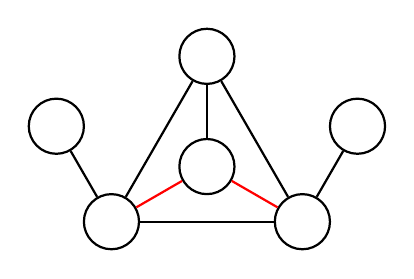
\begin{tikzpicture}
  [scale=1,normalN/.style={circle,draw,minimum size=0.7cm,thick}]

  \node[normalN] (center) at (0:0)    {};
  \node[normalN]   (top)    at (90:1.4) {};
  
  \path (210:1.4) node[normalN]   (left) {}
       +(120:1.4) node[normalN] (l)    {};
  

  \path (-30:1.4) node[normalN]   (right) {}
       +(60:1.4)  node[normalN] (r)     {};
  
  \draw [thick] (center) -- (top);
  \draw [thick,red] (center) -- (left);
  \draw [thick,red] (center) -- (right);
  
  \draw [thick] (left) -- (right);
  \draw [thick] (top) -- (right);
  \draw [thick] (top) -- (left);

  \draw [thick] (left)  -- (l);
  \draw [thick] (right) -- (r);
  
\end{tikzpicture}
\caption{Die zu viel eingezeichneten Kanten (rot)}
\label{pic:wrongEdges}
\end{figure}

Durch diese Kanten ist der gemeinsame (induzierte) Teilgraph nicht korrekt dargestellt. Abbildung \ref{pic:correctGraphs} stellt die korrekten Graphen für die Abbildungen~2.2b und 2.3b dar.

\begin{figure}[htb]
\centering
\hspace*{\fill}
\subfloat[Der Graph für Abb. 2.2b]{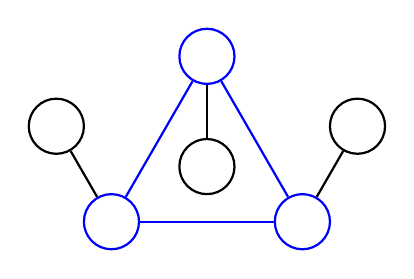
\begin{tikzpicture}
  [normalN/.style={circle,draw,minimum size=0.7cm,thick},
   blueN/.style={normalN,blue}]

  \node[normalN] (center) at (0:0)    {};
  \node[blueN]   (top)    at (90:1.4) {};
  
  \path (210:1.4) node[blueN]   (left) {}
       +(120:1.4) node[normalN] (l)    {};
  

  \path (-30:1.4) node[blueN]   (right) {}
       +(60:1.4)  node[normalN] (r)     {};
  
  \draw [thick] (center) -- (top);
  %\draw [thick] (center) -- (left);
  %\draw [thick] (center) -- (right);
  
  \draw [thick,blue] (left) -- (right);
  \draw [thick,blue] (top) -- (right);
  \draw [thick,blue] (top) -- (left);
  
  \draw [thick] (left)  -- (l);
  \draw [thick] (right) -- (r);
\end{tikzpicture}}
\hspace*{\fill} 
\subfloat[Der Graph für Abb. 2.3b]{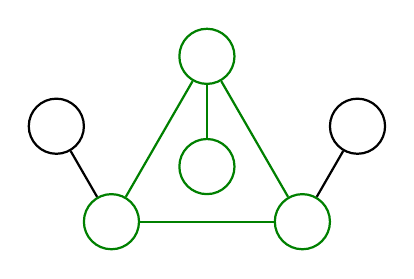
\begin{tikzpicture}
  [normalN/.style={circle,draw,minimum size=0.7cm,thick},
   blueN/.style={normalN,darkgreen}]

  \node[blueN] (center) at (0:0)    {};
  \node[blueN]   (top)    at (90:1.4) {};
  
  \path (210:1.4) node[blueN]   (left) {}
       +(120:1.4) node[normalN] (l)    {};
  

  \path (-30:1.4) node[blueN]   (right) {}
       +(60:1.4)  node[normalN] (r)     {};
  
  \draw [thick,darkgreen] (center) -- (top);
  %\draw [thick] (center) -- (left);
  %\draw [thick] (center) -- (right);
  
  \draw [thick,darkgreen] (left) -- (right);
  \draw [thick,darkgreen] (top) -- (right);
  \draw [thick,darkgreen] (top) -- (left);
  
  \draw [thick] (left)  -- (l);
  \draw [thick] (right) -- (r);
\end{tikzpicture}}
\hspace*{\fill}
\caption{Die korrekten Graphen für Abbildung 2.2b und 2.3b}
\label{pic:correctGraphs}
\end{figure}

\section*{Abbildung 2.4b}
Bei Abbildung 2.4b ist die Beschriftung der Knoten falsch. Statt $a$, $b$, $c$ und $d$ ist die korrekte Beschriftung $1$, $2$, $3$ und $4$. Abbildung \ref{pic:correctGraphs} stellt den Graphen aus Abb.~2.4b mit korrekter Beschriftung dar.

\begin{figure}[htb]
\centering
\hspace*{\fill} 
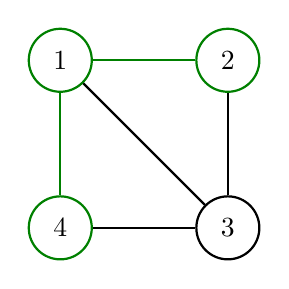
\begin{tikzpicture}
  [normalN/.style={circle,draw,minimum size=0.8cm,thick},
   greenN/.style={circle,draw=darkgreen,minimum size=0.8cm,thick},
   node distance=1.3cm]

  \node[greenN] (a) {1};
    
  \node[greenN] (b) [right=of a] {2}
    edge [thick,darkgreen] (a);
    
  \node[normalN] (c) [below=of b] {3}
    edge [thick] (b)
    edge [thick] (a);
    
  \node[greenN] (d) [left=of c] {4}
    edge [thick,darkgreen] (a)
    edge [thick] (c);
  
\end{tikzpicture}
\hspace*{\fill} 
\caption{Der Graph aus Abb.~2.4b mit korrekter Beschriftung}
\label{pic:bspMCS_GED}
\end{figure}

\bibliography{korrektur}

\end{document}
